\documentclass[10pt]{beamer}

\usetheme[progressbar=frametitle]{metropolis}

\usepackage{booktabs}
\usepackage[scale=2]{ccicons}

\usepackage[serbian]{babel}
\usepackage[T1]{fontenc}
\usepackage[utf8]{inputenc}
\usepackage{subcaption}


\usepackage{pgfplots}
\usepgfplotslibrary{dateplot}

\usepackage{xspace}
\newcommand{\themename}{\textbf{\textsc{metropolis}}\xspace}

\title{Implementacija AXI periferije na FPGA čipu}
\subtitle{Diplomski rad}
\date{septembar 2016}
\author{Lazar Caković}
\institute{Univerzitet u Beogradu, Elektrotehnički fakultet, Beograd}
\titlegraphic{\hfill\includegraphics[height=1.7cm]{images/ETF.png}}

\begin{document}

\maketitle

\begin{frame}{Sadržaj}
  \setbeamertemplate{section in toc}[sections numbered]
  \tableofcontents[hideallsubsections]
\end{frame}

\section{Uvod}

\begin{frame}[fragile]{Uvod}

	Integrisan sistem (embedded system) je računarski sistem specijalne namene koji je dizajniran da obavlja veoma male skupove aktivnosti.

	\bigskip	
	
	Integrisani sistemi se koriste od prenosnih uređaja (digitalnih satova, moblinih telefona, \dots), preko većih sistema kao što su saobraćajni semafori, kontroleri u fabrikama, pa sve do kompleksnih sistema kao što su magnetna rezonanca, hibridna vozila, \dots
	
\end{frame}
\begin{frame}[fragile]{Zamisao}
  
	Zamisao je da se napravi jedna periferija, koja će implementirati jednostavne stvari, ali koja će potpuno i pouzdano raditi taj mali set aktivnosti.
	
	\bigskip
	
	Periferija je AXI4-Lite, kako bi se pokazale mogućnosti AXI protokola.
	
	\bigskip
	
	Ova jednostavna periferija je zamišljena da radi uz pomoć Linux Kernel-a.
	
	\bigskip	
	
	Cilj je da se pokaže jedan ceo proces, uz teorijsku osnovu i propratne komentare, od zamisli do realizacije i korišćenja uređaja.
  
\end{frame}

\section{Hardware}

\begin{frame}{Hardverska realizacija}
	
	Hardversko okruženje ZC702, proizvođača Xilinx.
	
	\bigskip
		
	\begin{figure}[htb]
		\centering
		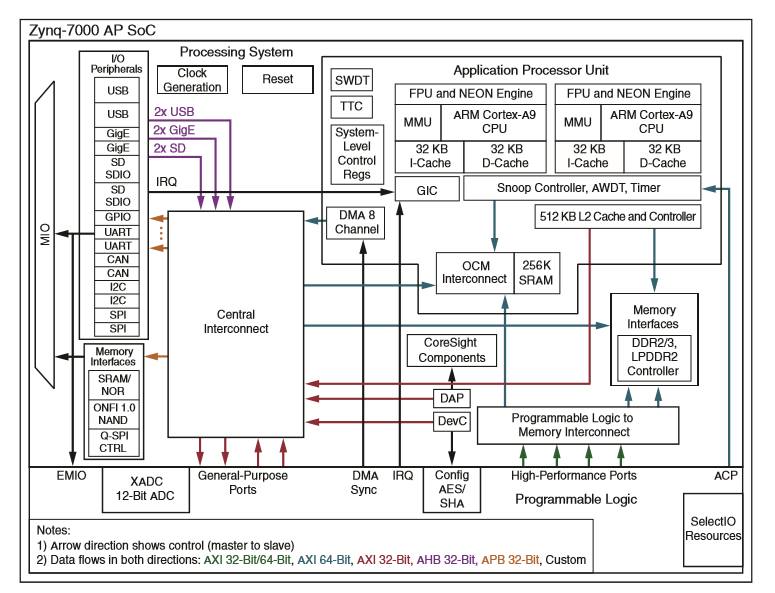
\includegraphics[width=.6\textwidth]{images/ZYNQ7000BD.png}
		\caption{Blok dijagram XC7Z020 AP SoC}
		\label{fig:zynq}
	\end{figure}	
		
	
\end{frame}

\begin{frame}{ZYNQ-7000}
	
	Zynq-7000 XC7Z020-1CLG484C AP SoC (All Programmable System On Chip)
	
	\bigskip
	
	\begin{figure}[htb]
		\centering
		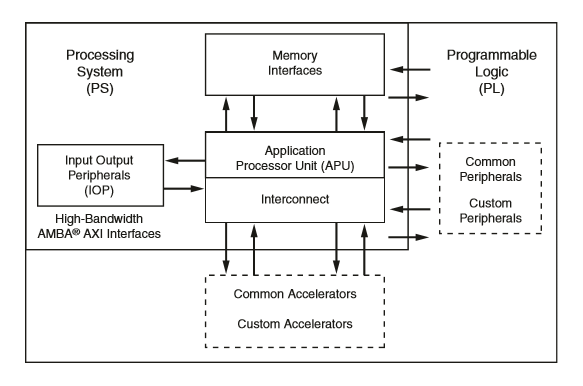
\includegraphics[width=.7\textwidth]{images/PSZYNQ7000.png}
		\caption{Blok dijagram procesorskog sistema i programabilne logike}
		\label{fig:procSysProgLog}
	\end{figure}
	
\end{frame}

\section{AXI}

\begin{frame}{AXI uvod}
	
	Advanced eXtensible Interface (AXI) je deo ARM AMBA(Advanced Microcontroller Bus Architecture) familije magistrala za mikrokontrolere.
	
	\bigskip
	
	Trenutno postoje tri tipa interfejsa koji rade sa AXI4 protokolom:

	\begin{itemize}
	
		\item AXI4 – za potrebe memorijski mapiranih uređaja visokih performansi.
		\item AXI4-Lite – za jednostavnu memorijski mapiranu komunikaciju (kao na primer za čitanje i upis u statusne i kontrolne registre).
		\item AXI4-Stream – za obradu podataka koji dolaze velikom brzinom.
		
	\end{itemize}
	
\end{frame}

\begin{frame}{Arhitektura AXI}
	
	\begin{figure}
		\centering
		\begin{subfigure}{.5\textwidth}
  			\centering
 			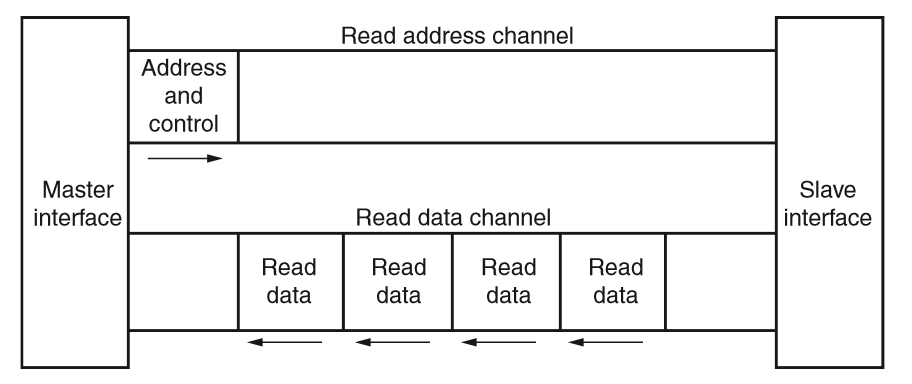
\includegraphics[width=.75\linewidth]{images/axireadprotocol.png}
  			\caption{AXI Read}
  			\label{fig:axiRead}
		\end{subfigure}%
		\begin{subfigure}{.5\textwidth}
  			\centering
  			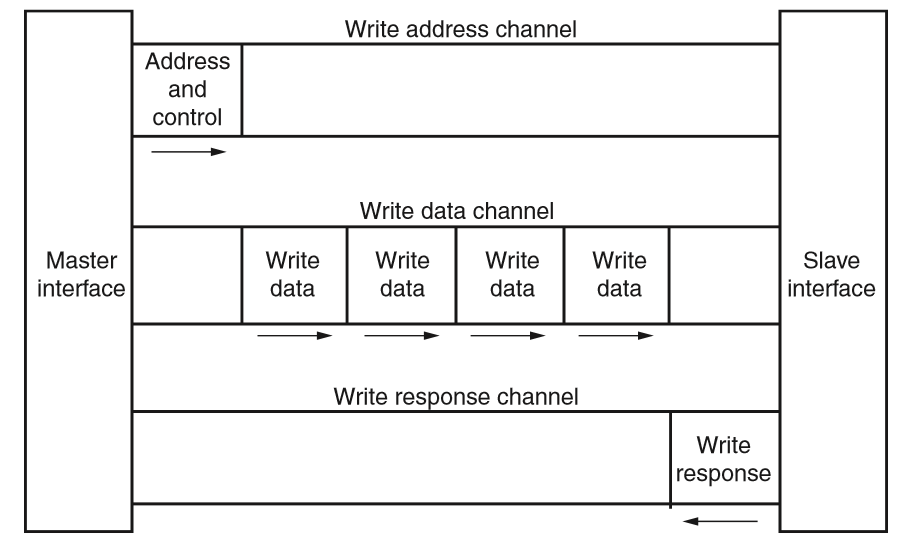
\includegraphics[width=.75\linewidth]{images/axiwriteprotocol.png}
  			\caption{AXI Write}
  			\label{fig:axiWrite}
		\end{subfigure}
		\caption{AXI protokol za čitanje i pisanje izmedju mastera i slejva}
		\label{fig:axiProtocol}
	\end{figure}
	
	Svaki od pet nezavisnih kanala se sastoji od seta informacionih signala i koristi dvosmerne \textit{VALID} i \textit{READY} mehanizme rukovanja (\textit{handshake mechanism}).
	
\end{frame}

\begin{frame}{AXI periferija}

	Na slikama je prikazana sa jedne strane AXI periferija koja je napravljena, dok je sa druge strane prikazan način na koji je periferija uključena u sistem koji je implementiran na čipu ZYNQ-7000.
	
	
	\begin{figure}
		\centering
		\begin{subfigure}{.5\textwidth}
  			\centering
 			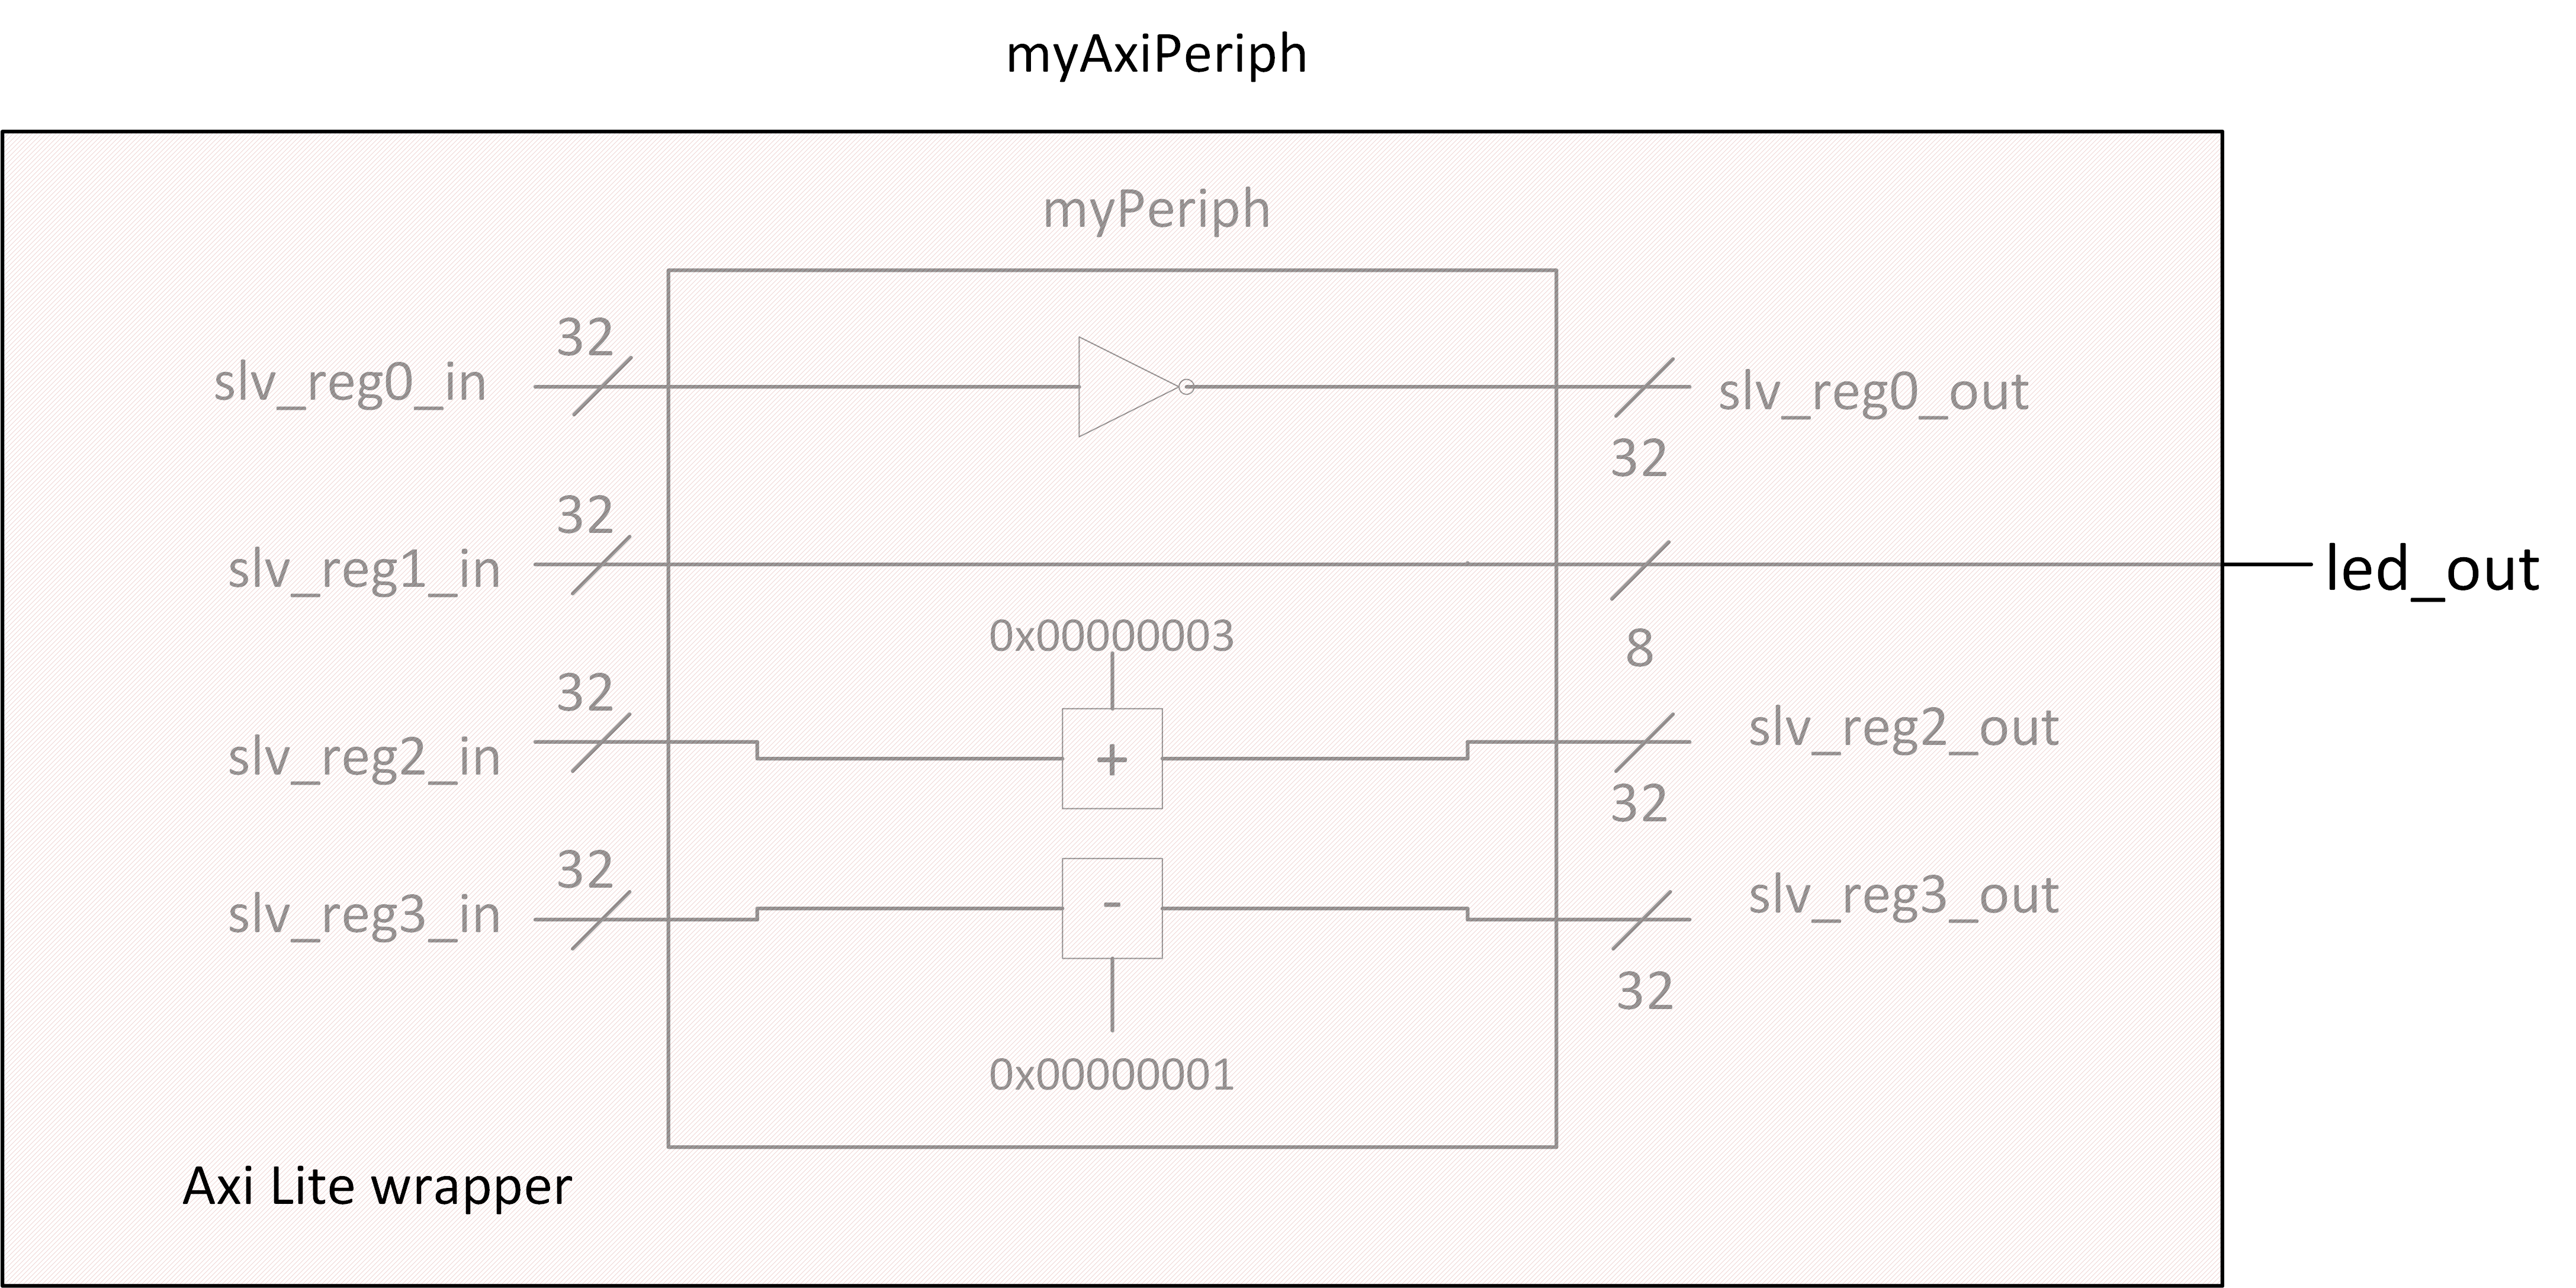
\includegraphics[width=.75\linewidth]{images/myaxiperiph.png}
  			\caption{Periferija ugrađena u AXI4-Lite}
  			\label{fig:axiPeripheral}
		\end{subfigure}%
		\begin{subfigure}{.5\textwidth}
  			\centering
  			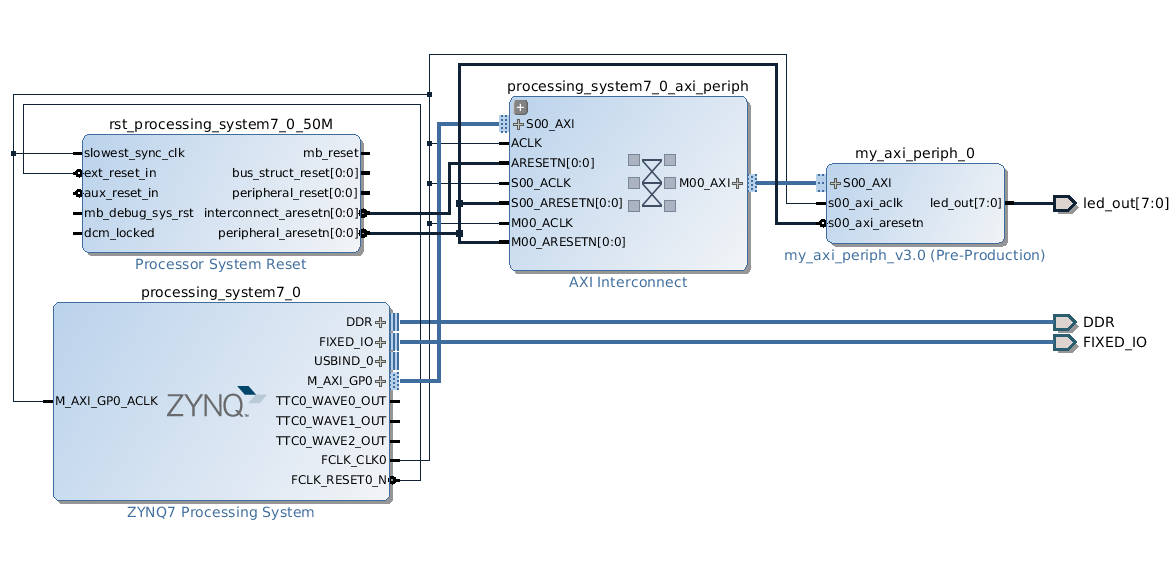
\includegraphics[width=.9\linewidth]{images/zc702system_vivado.png}
  			\caption{ZYNQ sistem}
  			\label{fig:zynqSystem}
		\end{subfigure}
		\caption{Periferija i sistem napravljen u Xilinx Vivado alatu}
		\label{fig:axiSystem}
	\end{figure}
	
\end{frame}


\section{Linux}

\begin{frame}{Linux uvod}
	
	Linux je jezgro operativnih sistema nalik UNIX-u. Kernel Linux-a je osmilio i napisao Linus Torvalds 1991. godine za ličnu upotrebu.
	
	\bigskip	
	
	Kernel se sastoji od delova za upravljanje procesima, upravljanje memorijom, fajl sistema, kontrole uređaja i komunikacije.
	
	
\end{frame}

\begin{frame}{Linux driver}

		Drajveri imaju posebnu ulogu u kernelu. Oni su odvojene crne kutije koje čine da jedan deo hardvera odgovara na zadat način i prema zadatom interfejsu, i time sakrije kako uređaj radi.
	
		\bigskip	
	
		Modularnost kernel - a i klase uređaja unutar Linux - a.
		
		\bigskip		
		
		Razlika između kernel modula i aplikacija.
		
\end{frame}

\begin{frame}{Linux}
	
	User space vs. Kernel space.
	
	\bigskip	
	
	File systems.	
	
\end{frame}

\section{Software}

\begin{frame}{Zamisao izrade}
	
	Jedna jednostavna periferija koja će raditi u svakom trenutku i biti uključena u kompjuterski sistem.
		
\end{frame}

\begin{frame}{Izrada}
	
	Boot Linux - a na ploču zc702, priprema i realizacija.
	
	\bigskip	
	
	Priprema fajlova za ispravnu inicijalizaciju Linux - a.
	
\end{frame}

\begin{frame}{Linux driver}
	
	Sam drajver je napisan koristeći mogućnosti /proc fajl sistema i struktura kernela.	
	
	\bigskip	
	
	\begin{itemize}
	
		\item \textit{file\_operations}
		\item \textit{file}
		\item \textit{inode}
		
	\end{itemize}	
	
	\bigskip
	
	Predefinisane funkcije.
	
\end{frame}

\begin{frame}{Application}
	
	Softverska aplikacija koja se dostavlja korisniku uz periferiju.
	
	\bigskip	
	
	Distanciranje korisnika od načina izrade.
	
\end{frame}


\section{Zaključak}

\begin{frame}{Zakljucak}
	
	Šta je postignuto ovim?
		
	\bigskip		
		
	Kako je moguće unaprediti izrađenu periferiju i softverski sistem?
	
\end{frame}

\begin{frame}[standout]
  Pitanja?
\end{frame}

\end{document}
